% Sección del artículo — dueño: P5. Sólo el dueño edita este archivo (v18).
\subsection{Formulación y funciones de pérdida}
La mosca minimiza la entropía cruzada ponderada por clase sobre las acciones del experto,
\begin{equation}
\mathcal{L}_{\text{mosca}}(\theta) = -\frac{1}{N}\sum_{i=1}^{N}\sum_{c=1}^{C}
w_c\, y_{i,c}\log p_\theta(c \mid x_{i,t-T+1:t}, g_i)
\label{eq:mosca}
\end{equation}
y la abeja la pérdida~\eqref{eq:abeja}.

\subsection{Entrenamiento y métricas}
Las redes de la mosca se entrenan por clonación de comportamiento sobre las etiquetas del
experto, minimizando la entropía cruzada ponderada~\eqref{eq:mosca} con $w_c\propto f_c^{-1/2}$
(recortado a 10), pues las acciones están desbalanceadas (40\,\% \emph{avanzar} y
0.1\,\% \emph{mantener posición}). Se usa AdamW~\cite{loshchilov2019} (tasa $10^{-3}$, decaimiento de pesos
$10^{-4}$, programación coseno), lotes de 256, hasta 15 épocas con parada temprana
(paciencia 4) y se conserva el modelo con mejor F1 macro en validación; el conjunto de
prueba no interviene en ninguna decisión. Los gradientes se recortan a norma 1. Cada
configuración se entrena con 3 semillas. La abeja usa el mismo optimizador con lotes de 512,
hasta 30 épocas con paciencia 6 sobre el error angular mediano de validación y un aumento que
rota la vista actual $\pm1$ sector (error de brújula de $\pm5$\textdegree).

Para mitigar el desplazamiento de distribución de la clonación de comportamiento se
aplica DAgger~\cite{ross2011} (Fig.~\ref{fig:dagger}): en la iteración $k$ la política
ejecutada es $\pi_k=\beta_k\pi^*+(1-\beta_k)\hat\pi_{k-1}$ con
$\beta=(0.5,\,0.25,\,0)$, el experto $\pi^*$ etiqueta los estados visitados, el conjunto
se agrega ($\mathcal D\leftarrow\mathcal D\cup\mathcal D_k$, 120 escenarios nuevos de
entrenamiento por iteración) y la red se reentrena 5 épocas desde los pesos anteriores.

\begin{figure}[t]
\centering
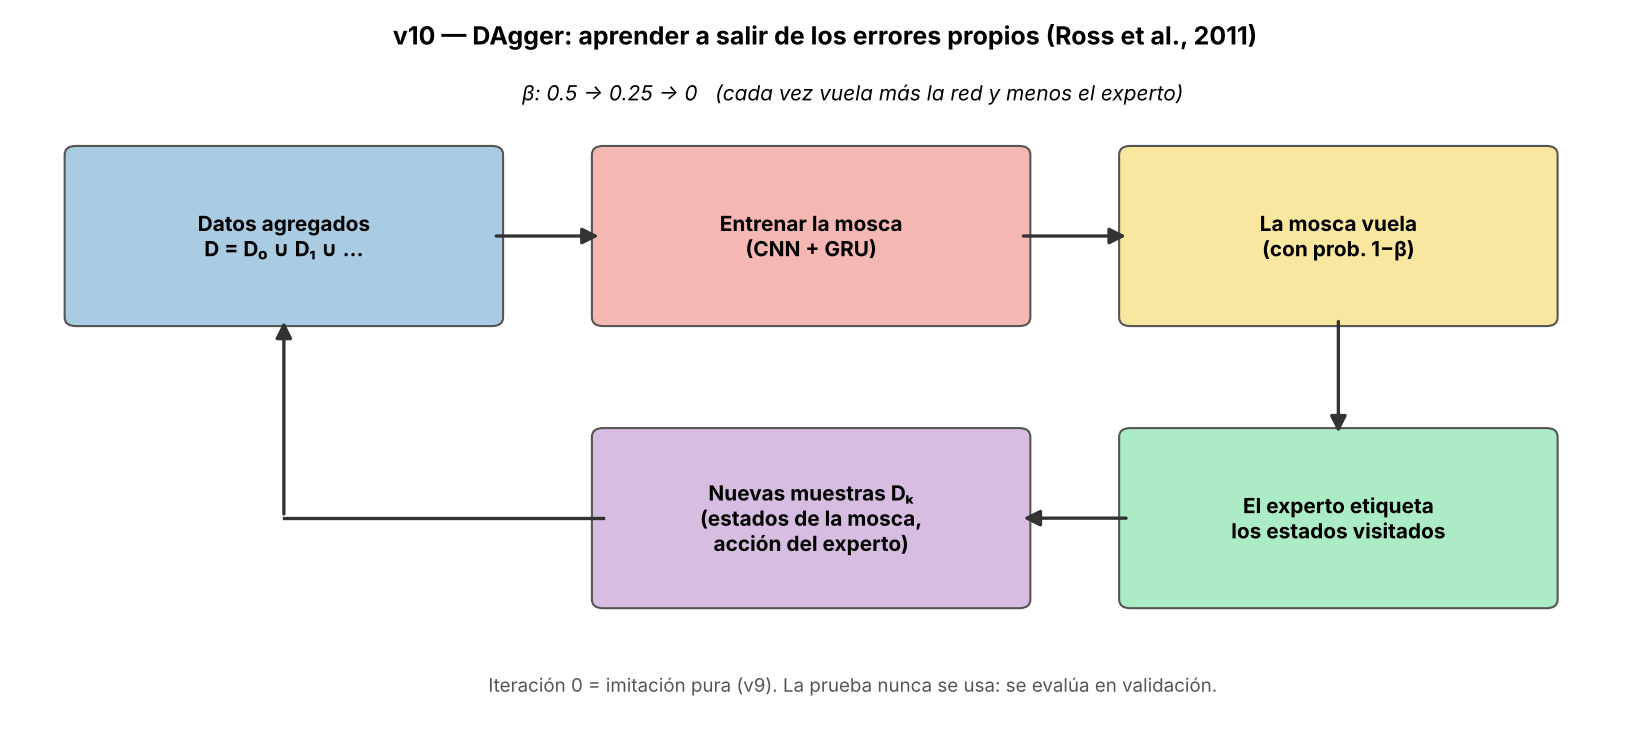
\includegraphics[width=\linewidth]{v10_dagger_esquema}
\caption{Ciclo de DAgger aplicado al módulo mosca.}
\label{fig:dagger}
\end{figure}
\textbf{Métricas.} Fuera de línea se reporta el F1 macro de validación, adecuado para
clases desbalanceadas (la exactitud premiaría avanzar siempre), y el AUROC macro uno contra
el resto~\cite{fawcett2006}, que mide si la red ordena bien las acciones con independencia del
umbral. La abeja se mide en grados (error angular mediano y fracción de vistas con error
$\le30$\textdegree), en la partición de prueba. En lazo cerrado, sobre las
semillas de prueba, se reportan la tasa de éxito de misión con su intervalo de Wilson al
95\,\%, la tasa de choques, el error de aterrizaje respecto de la base y la latencia por
decisión; para los controladores neuronales, la media $\pm$ desviación estándar entre las tres
semillas de entrenamiento.

\textbf{Significancia.} Como todos los controladores vuelan los mismos escenarios, las
comparaciones son pareadas: para cada escenario se toma el éxito de A y de B (media entre
semillas en los neuronales) y se analiza la diferencia $d_i$. Se reporta la media de $d_i$
con un IC 95\,\% bootstrap que remuestrea escenarios~\cite{efron1993}, el valor $p$ de una
prueba de permutación por cambio de signo (exacta, equivalente a McNemar, cuando $d_i\in\{-1,0,1\}$),
corregido por Holm~\cite{holm1979} sobre todas las comparaciones, y la $h$ de
Cohen~\cite{cohen1988} como tamaño de efecto.
